\section{Evaluering mot kravspesifikasjon}
\label{sec:evaluering}

Evalueringen av VideoAPI mot kravspesifikasjonen bygger på tre
uavhengige kilder: desgin og implementasjonen dokumentert i 
kapittel~\ref{ch:design} og~\ref{ch:implementasjon}, 
testresultatene i kapittel~\ref{ch:testing}, og en 
sluttevaluering fra HDO. Sluttevalueringen ble innhentet som et 
spørreskjema besvart av to representanter fra 
oppdragsgiver etter overlevering, og gir ekstern validering av 
at leveransen møter behovet i kravspesfiksjonen. Skalaen var 
1--5, der 5 indikerer at kravet er fullstendig oppfylt.
Fullstendige svar er gjengitt i 
vedlegg~\ref{app:hdo-eval}.

Figur~\ref{fig:hdo-eval-summary} oppsummerer HDOs vurderinger 
per kravområde.

\begin{figure}[h]
    \centering
    % Søylediagram (pgfplots): HDOs sluttevaluering per kravområde.
% Tallene er gjennomsnitt av respondentene; kilden er tabell~\ref{tab:hdo-eval-full} i vedlegg~\ref{app:hdo-eval}.
% Brukes typisk via \texttt{figures/hdo-eval-sammendrag.tex} i hovedteksten.
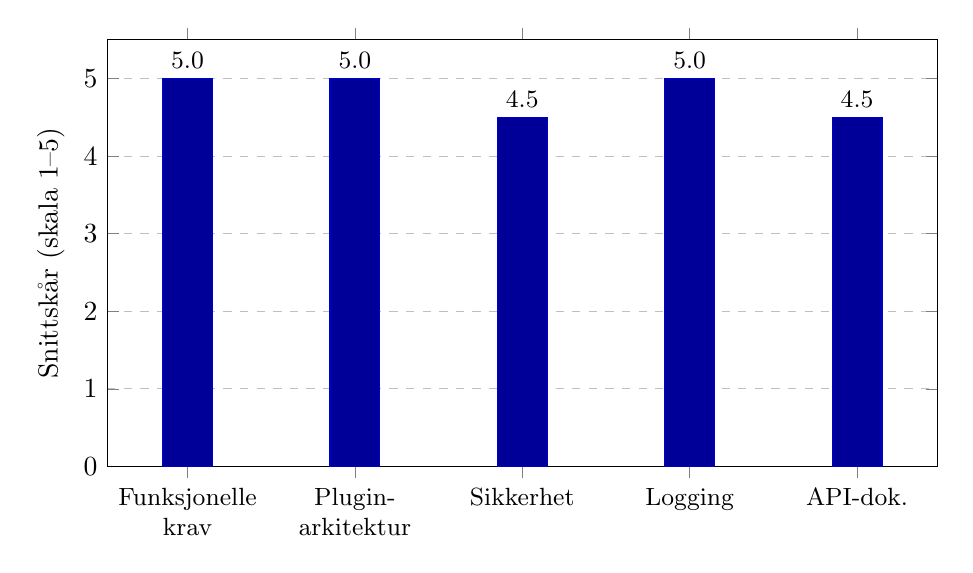
\begin{tikzpicture}
    \begin{axis}[
        width=\linewidth,
        height=7cm,
        ybar,
        bar width=18pt,
        ymin=0,
        ymax=5.5,
        ytick={0,1,2,3,4,5},
        ylabel={Snittskår (skala 1--5)},
        symbolic x coords={
            {Funksjonelle\\krav},
            {Plugin-\\arkitektur},
            {Sikkerhet},
            {Logging},
            {API-dok.},
            {Samlet\\leveranse}
        },
        xtick=data,
        xticklabel style={
            align=center,
            font=\small,
            text width=2cm
        },
        nodes near coords,
        nodes near coords style={font=\small},
        every node near coord/.append style={
            /pgf/number format/.cd,
            fixed,
            fixed zerofill,
            precision=1
        },
        enlarge x limits=0.12,
        ymajorgrids=true,
        grid style=dashed,
    ]
        \addplot[
            fill=blue!60!black,
            draw=blue!80!black
        ] coordinates {
            ({Funksjonelle\\krav},5.0)
            ({Plugin-\\arkitektur},5.0)
            ({Sikkerhet},4.5)
            ({Logging},5.0)
            ({API-dok.},4.5)
        };
    \end{axis}
\end{tikzpicture}

    \caption{HDOs sluttevaluering av VideoAPI per kravområde, 
    snittskår på skala 1--5.}
    \label{fig:hdo-eval-summary}
\end{figure}

\subsection{Funksjonelle krav (F1.1--F1.5)}
\label{sec:eval-funksjonelle}

% Oppfyllelse av funksjonelle krav

\subsection{Sikkerhetskrav (S1.1--S1.2)}
\label{sec:eval-sikkerhet}

% Oppfyllelse av sikkerhetskrav

\subsection{Infrastrukturkrav (I1.1--I1.2)}
\label{sec:eval-infrastruktur}

% Oppfyllelse av infrastrukturkrav

\subsection{Observability-krav (O1.1--O1.3)}
\label{sec:eval-observability}

% Oppfyllelse av observability-krav
